\documentclass{scrartcl}
\usepackage[utf8]{inputenc}
\usepackage{polski}
\usepackage{amsmath}
\usepackage{graphicx}

\title{UKS de La Salle.}
\subtitle{Modernizacja serwisu.}
\author{Tomasz Szymanek
\and
Tomasz Żubertowski}

\date{2013-2014}

\usepackage{natbib}
\usepackage{graphicx}

\begin{document}

\maketitle

\section{UKS de La Salle}
W ramach projektu zespołowego na Uniwersytecie Gdańskim chcemy podjąć się modernizacji serwisu (we współpracy z JIT Solutions):
http://uksdelasalle.pl/.
\section{Aspekty prawne}
\subsection{Fonty/Czcionki}
Aby nie przeciążać hostingu i zniwelować problem roszczeń co do praw autorskich d/t czcionek planujemy bazować jedynie na czcionkach dostępnych na licencji Open Source, najprawdopodobniej wyłącznie z serwisu: 
http://www.google.com/fonts.
\subsection{Zdjęcia, obrazy, stocki}
Sprawa z obrazami ma się prościej aniżeli z czcionkami. Wszystkie zdjęcia i obrazy będą pochodzić ze źródeł uczniowskiego klubu sportowego UKS de La Salle. Ewentualne grafiki użyte w serwisie będą wygenerowane albo przy użyciu css, albo będą posiadały licencję Open Source.
\subsection{Technologia/narzędzia pracy}
Nie będziemy korzystać z gotowych rozwiązań w postaci skryptów, czy całych silników cms ( : ) ). Ponadto wszystkie narzędzia: edytory tekstu, edytory grafiki, których użycie zaplanowaliśmy są darmowe do użytku komercyjnego, bądź też posidamy do nich licencje.

\section{Wykonanie, koncept}
Trendy webdesignu dyktują prawa co do których będziemy starać się projektować tę modernizację. Popularne serwisy internetowe takie jak np.: allegro.pl, ceneo.pl, gazeta.pl, czy nawet serwisy zagraniczne: cinemassacre.com, gametrailers.com, a nawet aplikacje mobilne stawiając na minimalizm w przekazie uzyskują czytelność. 

\begin{figure}
  \centering
  
\includegraphics[width=1\linewidth]{TCN4mWO.png}
  \captionof{figure}{Design allegro.pl}
  \label{fig:test1}
\end{figure}
\begin{figure}
  \centering
  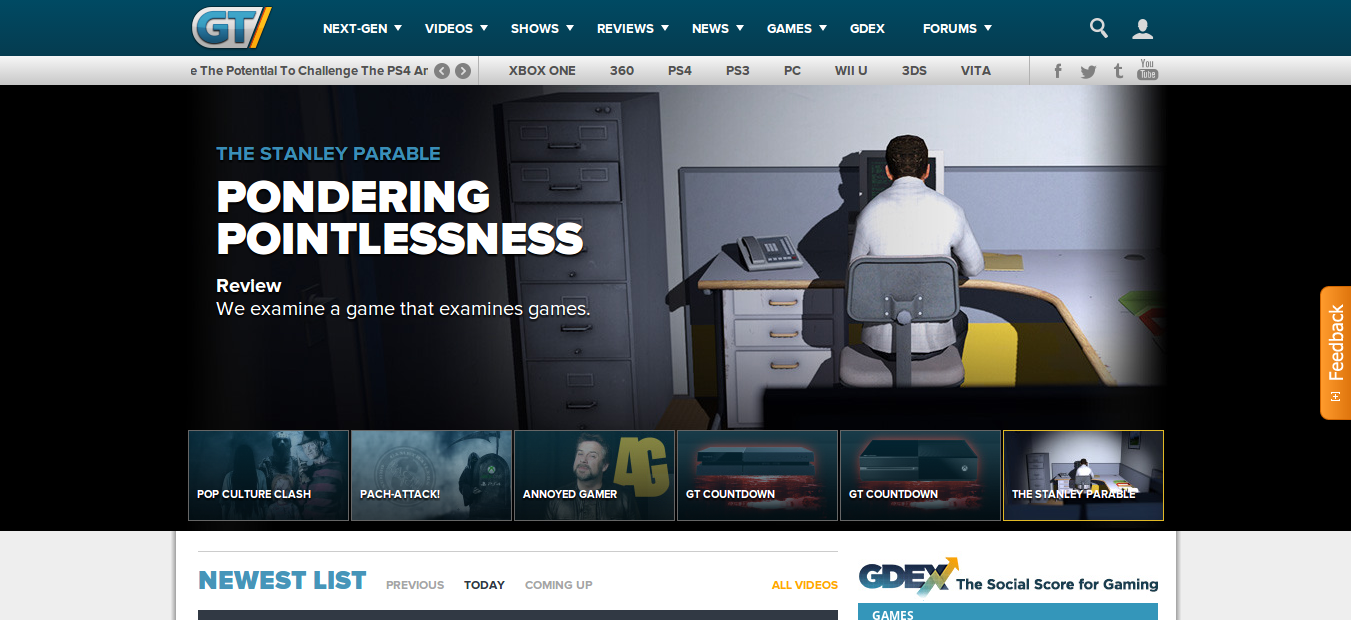
\includegraphics[width=1\linewidth]{vTHA7wq.png}
  \captionof{figure}{Design gametrailers.com}
  \label{fig:test2}
\end{figure}

\section{Koncept}
\subsection{Strona główna}
Strona główna składa się z czterech stałych elementów - topu, tam gdzie znajdzie się menu kontekstowe.
\subsubsection{Nagłówek}
W górnej części strony zamierzamy umieścić logo UKS oraz element umożliwiający wyszukiwanie treści. Poniżej znajdować się będzie menu kontekstowe w formie odnośników do poszczególnych sekcji sportowych.

Każdy z elementów menu będzie logiem, umieszczenie kursora myszy nad daną sekcją rozwija podmenu dotyczące w/w.
\subsubsection{Slider i kalendarz} 
Najciekawszym elementem naszego pomysłu jest slider, który zawierać będzie informacje dotyczące najnowszych postów z każdej sekcji. Zdjęcia do newsów znajdujące się na sliderze umożliwiać będą przejście na podstronę danej sekcji i załadowanie danego artykułu.

Elementem sąsiadującym ze sliderem będzie kalendarz zawierający nadchodzących X wydarzeń (dla każdej sekcji po jednym) z datą wydarzeń, godziną oraz nazwą.
\subsubsection{Wiadomości}
Ta część strony poświęcona będzie wiadomościom dotyczącym klubu oraz po odpowiednim wybraniu sekcji - wiadomościom i każdej innej grupie artykułów dotyczącym danej sekcji. 
\subsubsection{Stopka}
Stopka jest elementem stałym niezależnie od wybranej sekcji, podzielona zostanie na dwie części. Informacje zawarte w pierwszej nawiązują stricte do UKS jako organizacji nonprofit. Ponadto jest kolejne miejsce nawigacyjne do danej podsekcji, gdzie nawigacja polega na wybraniu odnośnika do danej sesji.

Druga część stopki to wszelkiej maści informacje kontaktowe wraz z ewentualną dynamiczną częścią w postaci adresu/mapy dojazdu.

\subsection{Technologie}
\subsection{Frontend/backend}
Jako, że projekt jest realizowany w związku z zajęciami uczelnianymi planujemy nie korzystać z gotowych rozwiązań ani co do backendu, ani frontendu. Przykładowo - zamiast korzystać z bootstrapa sami będziemy rozwijać część cssową.  Naturalnym rzecz jasna jest jednak wzorowanie się na rozwiązaniach przyjętych przez rynek.
\subsubsection{Nagłówek}
\paragraph{Frontend}
Logo UKS będzie statyczne, część wyszukiwania będzie realizowana przez PHP i będzie obejmować cały serwis wraz z podstronami sekcji.
\paragraph{Backend}
Backend nagłówna sprowadza się do przekazania zapytania do PHP i wyszukiwania po bazie danych.
\subsubsection{Slider}
\paragraph{Frontend}
Sam frontend Slidera wraz z kalendarzem będzie zrealizowany w technologii opartej na JavaScript i CSS.
\paragraph{Backend}
Treści slidera będą dynamicznie dopasowywane po wynikach z zapytań do bazy SQL, rzecz jasna za pomocą PHP. 
\subsubsection{Body}
\paragraph{Frontend}
Wiadomości to jednak praktycznie sam backend, frontend podobnie jak w przypadku Slidera i kalendarza będzie oparty o JavaScript i CSS. Treści podstron/sekcji będą dostarczane w sposób dynamiczny, prawdopodobnie przy użyciu AJAX/angularJS/JQuery.
\paragraph{Backend}
Po wybraniu sekcji część Slidera zniknie lub zostanie dostosowana do danej sekcji. Ponownie: dane ewentualnie wypełniające slider będą pobierane za pomocą zapytań do SQL przez PHP, a wypełniane JQuery/JS/angularJS.

Po wybraniu sekcji i zmianie części Slidera następuje czas na dynamiczne przypisanie treści wiadomości pod kątem wybranej sekcji. Pragnę podkreślić, że strona nie będzie się przeładowywać przy zmianie kategorii/sekcji, wszystko będzie realizowanie dynamicznie (angularJS/JQuery). Przy wyborze terminarza w sekcji wiadomości wyświetla się kalendarz wydarzeń. 

\subsubsection{Stopka}
\paragraph{Frontend}
Jedynym dynamicznym elementem będą treści kontaktowe. Ponownie kładziemy nacisk na AJAX/angularJS/JQuery.
\paragraph{Backend}
Przy wykonaniu elementu dynamicznego dt. informacji kontaktowych dalej stawiamy na JS/angularJS/PHP.



\bibliographystyle{plain}
\bibliography{references}
\end{document}


\subsection{}

\begin{figure}[h!]
  \caption{Porównanie czasów działania.}
  \centering
    \includegraphics[width=0.7\textwidth]{czas.png}
\end{figure}

\bibliographystyle{plain}
\bibliography{references}
\end{document}
